\subsubsection*{Visitor Pattern}\label{subs:visit}
The visitor pattern is not only used to traverse the parse tree provided by ANTLR, but also the \acrfull{ast}.
The visitor pattern is implemented throughout the compiler, to create the \acrshort{ast} from the parse tree and for traversing the \acrshort{ast}.
As such the visitor pattern defines the structure of the compiler, and thus understanding the benefit from using the pattern is important.
The visitor pattern is described by the Gang of Four, authors of ``Design Patterns: Elements of Reusable Object-Oriented Software'' as:
``a design pattern that separates a set of structured data from the functionality that may be performed upon it.''. \citep{GOF}

The pattern is a behavioral pattern i.e. it defines how communication between classes and entities are handled.
In the tree walk for the parse tree, the visitor should convert the parse tree into a \acrshort{ast}.
This entails that each different node in the parse tree must be visited to find the information needed to create the \acrshort{ast}.

Through use of the visitor pattern the functionality is separated from the classes they are performed upon. 
Instead the functionality is on a visitor class implementing the visitor interface, which means different visitors can be made, which all do different computations while traversing the tree.
Each class in the tree have an \texttt{accept} method that allows them to call the visitor in question with itself as an argument.
This allows the ability of adding new operations without changing the original data structure, and also without changing other visitors, an invaluable feature when doing iterative development.
Another benefit is that a single visitor object is used to visit all the classes in the tree.
This visitor can therefore maintain a state between calls to individual data objects, which can be used to save information in an outer scope from the different visit calls.
\myref{image:visitor} shows a UML diagram of the visitor pattern.
This diagram is from a C\# representation, and while the idea is the same the exact implementation is not identical to the one used in the compiler for GAMBLE.
Take note of are the classes ``ConcreteElement'' and ``ConcreteVisitor'', the ``ConcreteElement'' represents the different kinds of nodes in a given tree.
The ``ConcreteVisitor'' represent the different kind of visitors implemented.
A visitor will make sure that the children of the node is traversed in the correct way, and will at the same time also do other computations, e.g. pretty printing or checking the sourcecode for errors.
A visitor must implement a method to visit every single ``ConcreteElement'' which exist in the tree.
As can be seen on \myref{image:visitor} ``ConcreteVisitorA'' and ``ConcreteVisitorB'', both implement a visit method for the ``ConcreteElements'' A and B.
In the next section, the implementation of creating the \acrshort{ast} from the parse tree using the visitor pattern will be presented.

\begin{figure}[!ht]
\centering
 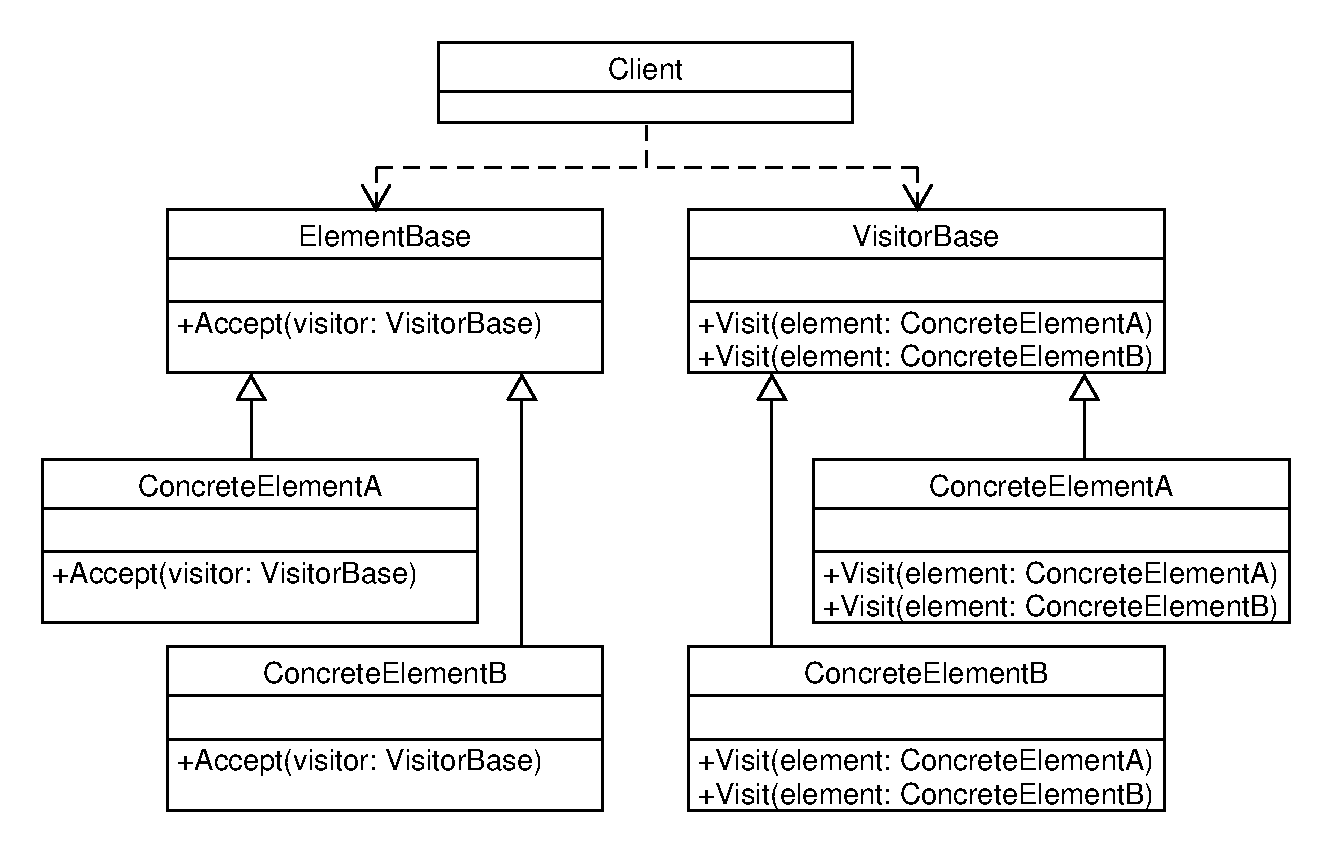
\includegraphics[width=1\textwidth]{figures/ClassDiagrams/VisitorPattern.pdf} % trim=4.85cm 15cm 0.85cm 1cm
\caption{A UML diagram for the implementation of the visitor pattern.}\label{image:visitor}
\vspace{-15pt}
\end{figure}


